\chapter{背景}
\label{background}

本章では本研究の背景について述べる.

\section{ネットワーク音楽演奏}
ネットワーク音楽演奏で演奏を届ける手法は,VoIPアプリケーションのように音声の波形情報を処理し低遅延で届ける方法\cite{syncroom}\cite{lola}\cite{jacktrip},演奏情報をMIDIを使い楽器,音程,強度などに抽象化し,受信した機器が演奏データを元に音を合成するという方法\cite{rtpmidi}\cite{sourcenode}と,2種類の手法に分けることができる.
本研究では演奏予測を扱いやすい後者の手法を用いる.

\section{ネットワーク音楽演奏システムの構造}

\section{演奏情報の表現}
本研究では演奏をMIDIの形式であらわし,演奏情報を伝達する.
MIDIとは

\section{Open Sound Control}
Open Sound Control (OSC)\cite{opensoundcontrol}はソフトやコンピュータ同士でリアルタイムの通信を行うためのプロトコルである.
元々ネットワークを経由した楽器の演奏を前提として開発されているためデータ型としてMIDIを使えるうえ,時刻タグ(OSC Time Tag)をメッセージとまとめて送ることで正確な音の再生のタイミングを送信者から指定することが可能である.
そのうえ,OSCは広く使われていてライブラリや実装が豊富であるため本研究のシステムで採用した.

\begin{figure}[htbp]
  \centering
  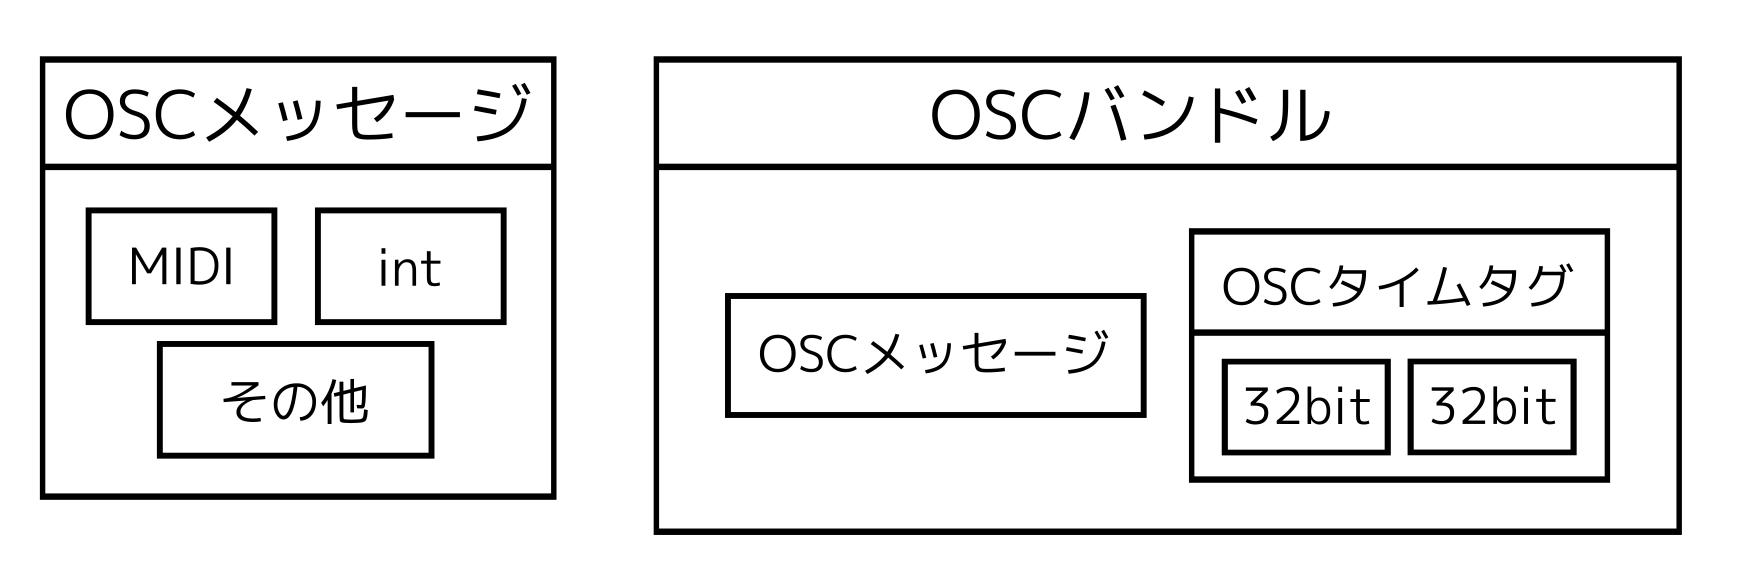
\includegraphics[width=0.8\linewidth]{src/img/g1736.png}
  \caption{OSCメッセージとOSCバンドル}
  \label{fig:oscmess}
\end{figure}

OSCのメッセージは単体で,もしくは時刻を指定して同時に再生する複数のメッセージをバンドルにまとめて送ることができる.
32ビットでUNIX時間での秒数を,32ビットで秒数の小数部を表す時刻タグをOSCで使用されるため高解像度で再生の管理が可能であり,時刻タグの精度は本研究では十分とする.

OSCサーバーがOSCメッセージやOSCバンドルを受信するとそれらを引数としてOSCメソッドが実行される.
OSCメソッドはOSCアドレス空間というツリー構造の中に配置され,OSCメッセージやOSCバンドルに付属されるOSCアドレスを宛先として実行されるOSCメソッドが選ばれる.

\section{Adaptive Metronome}
BattelloらによるAdaptive Metronome\cite{admet}\cite{admet:experiment}は,演奏者の演奏をリアルタイムで分析し,演奏者の演奏に合わせてメトロノームのテンポを変化させるシステムである.

\begin{figure}[htbp]
  \centering
  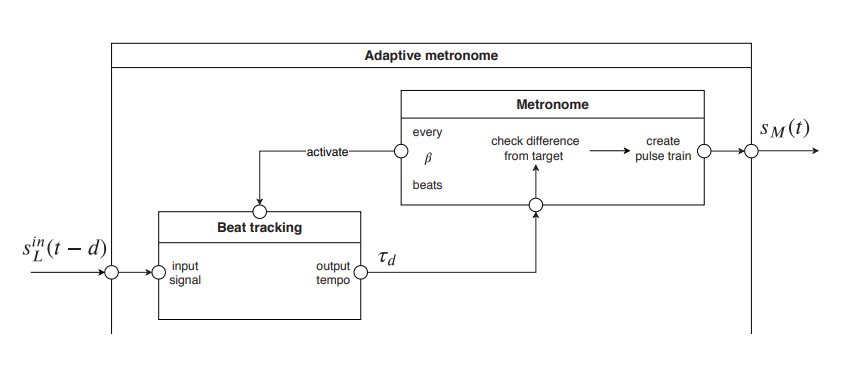
\includegraphics[width=0.8\linewidth]{src/admet.png}
  \caption{Adaptive Metronomeの実験\cite{admet}}
  \label{fig:admet}
\end{figure}

Adaptive Metronomeは親子構造を持っている.
親の演奏者は演奏すると同時にシステムはリアルタイムでその演奏の拍を推定し,子演奏者に音声と拍情報を送信する.
子演奏者のシステムはその情報を受取り,親演奏者の演奏に合わせてメトロノームのテンポを変化させる.
またこのときメトロノームの音は親から子への遅延を考慮して位相をずれして再生される.

こうすることで小演奏者に聞こえるメトロノームは親演奏者の遅延された演奏に関わらず,常に親演奏者の無遅延の演奏に合わせたテンポで再生される.
このシステムを用いた実験では120msの遅延下での演奏を行ったうえでも,被験者は抵抗を感じることなく演奏することができたという結果が得られた.\cite{admet}

\subsection{相互メトロノームの実験}
当初のAdaptive Metronomeの実験では,親演奏者の演奏を子演奏者が聴き,それに合わせて演奏するという形で実験が行われた.
後にBatteloらは親子構造を持たず,相互的にAdaptive Metronomeを聞きあう実験を行った.
実験の結果は現状まだ不十分であるが,このような相互的なシステムでもある程度の効果が得られることが示された.

\subsection{共通テンポの算出}
相互的にAdaptive Metronomeを聞きあう実験では,全体のテンポを決定させる親演奏者がいないため,演奏者同士のテンポと位相が異なる場合がある.
このとき2人の演奏者の状況を踏まえたうえで両方の演奏が同期するような共通のテンポを算出する必要がある.


% 以降は最後にメンション
\section{Tablanet}
Tablanet\cite{tablanet}は,タブラ奏者の演奏をリアルタイムで分析し,演奏者の演奏に合わせてタブラのテンポを変化させるシステムである.

\section{Alexandraki}
Alexandrakiらによる研究\cite{alexandraki:2013}\cite{alexandraki:2014}では,演奏者の演奏をリアルタイムで分析し,事前収録した演奏を実際の演奏に合わせて再生するシステムを提案している.
